\documentclass[conference]{IEEEtran}
\IEEEoverridecommandlockouts
\usepackage{cite}
\usepackage{amsmath,amssymb,amsfonts}
\usepackage{graphicx}
\usepackage{textcomp}
\usepackage{xcolor}
\usepackage{booktabs}
\usepackage{multirow}
\usepackage{url}

\def\BibTeX{{\rm B\kern-.05em{\sc i\kern-.025em b}\kern-.08em
    T\kern-.1667em\lower.7ex\hbox{E}\kern-.125emX}}

\begin{document}

\title{Model-Side Robustification of Monocular Metric Depth Estimation for Outdoor Mobile Robots:\\
A Reproduction and Extension of UniDepth V2 on KITTI}

\author{
\IEEEauthorblockN{Raja Haseeb Ahmad}
\IEEEauthorblockA{2025-MS-MC-01 --- Mobile Robotics, Final Project}
}

\maketitle

\begin{abstract}
Monocular metric depth estimation (MMDE) models such as UniDepth achieve strong zero-shot generalization across camera domains, but their behavior under the real-world sensor and environmental corruptions an outdoor mobile robot actually encounters -- rain, fog, low illumination, motion blur, and sensor noise -- is not addressed by the original work. This paper reproduces UniDepth V2 (ViT-L/14) on real KITTI outdoor sequences and studies its robustness under five degradation conditions motivated by established image-formation literature, at a small, single-GPU coursework scale (21 fine-tuning frames, 9 held-out frames from one KITTI drive). We first implement classical input-side image restoration as a candidate fix, then, per instructor-directed critical feedback, replace it with a model-side self-distillation fine-tuning strategy in which a frozen copy of the pretrained network supervises a partially-unfrozen decoder on degraded inputs, so that robustness is absorbed into the perception model itself rather than added as a preprocessing stage. Using a held-out evaluation protocol with fixed seeds and early stopping, we find a consistent, positive effect only for sensor noise (+6.5\%), with the remaining four conditions -- rain, fog, low light, and motion blur -- showing flat or mildly negative held-out effects at this scale, indicating that decoder-only self-distillation transfers unevenly across corruption types rather than uniformly improving robustness. We additionally report a single-scene demonstration metric that shows larger apparent gains for some conditions, and show this discrepancy traces to a peak-pixel measurement artifact rather than genuine robustness -- a methodological finding we argue is broadly relevant to small-scale depth-robustness studies. Finally, we implement a ROS2 Humble and Docker deployment architecture that serves either the original or a condition-specific fine-tuned checkpoint to a live camera topic, connecting the offline study to an onboard robotics pipeline; hardware-in-the-loop validation on a physical or simulated robot remains for future work.
\end{abstract}

\begin{IEEEkeywords}
monocular depth estimation, UniDepth, robustness, adverse weather, self-distillation, knowledge distillation, KITTI, mobile robotics, ROS2
\end{IEEEkeywords}

\section{Introduction}

Outdoor mobile robots rely on dense metric depth for obstacle avoidance, local planning, and terrain assessment. Monocular metric depth estimation (MMDE) is an attractive sensing modality because it needs only a single RGB camera, but it is also an ill-posed problem: depth must be inferred from appearance and learned priors rather than measured directly, as a stereo pair or LiDAR would. Recent foundation-style MMDE networks such as UniDepth \cite{ref1}, Metric3D \cite{ref4}, Depth Anything \cite{ref5}, and ZoeDepth \cite{ref3} have substantially closed the accuracy gap to metric sensors on curated benchmarks, and report strong zero-shot transfer across camera intrinsics and scene domains.

This generalization claim, however, concerns domain shift between clean datasets -- different cameras, indoor versus outdoor scenes -- and not the corruptions a physical robot's camera actually experiences during outdoor operation: rain streaking the lens or scene, atmospheric scattering in fog, underexposure at dusk or in shadow, motion blur from chassis vibration, and sensor noise from inexpensive or overheated hardware. Whether a state-of-the-art MMDE network remains reliable under these conditions -- and, if not, how to make it reliable without adding a fragile preprocessing stage to a real-time robotics pipeline -- is the practical question this project addresses.

The project began with input-side image restoration (deraining, dehazing, contrast enhancement, deconvolution, denoising) applied before the frozen depth network. Instructor feedback redirected the work toward a more architecturally meaningful question: rather than cleaning the image, can the depth model itself be made robust? We adopt a self-distillation fine-tuning strategy in which the model's own clean-image prediction supervises its degraded-image prediction, requiring no paired ground-truth depth and no external restoration network.

Contributions of this work:
\begin{itemize}
\item Reproduction of the UniDepth V2 (ViT-L/14) inference pipeline on real KITTI outdoor sequences, established as a clean baseline.
\item Five degradation conditions (rain, fog, low light, motion blur, sensor noise) motivated by the image-formation literature; rain and fog implement their cited physical models directly (Koschmieder veiling, depth-dependent transmission), while low light, motion blur, and sensor noise use simplified approximations (gamma darkening, isotropic blur, fixed-variance noise) of the cited phenomena, a simplification we note explicitly in Section~\ref{sec:degradation}.
\item A model-side self-distillation fine-tuning method, evaluated as an alternative to classical input-side restoration, directly responding to critical feedback received during development.
\item A held-out evaluation protocol (fixed seeds, train/test split, early stopping) that reveals a generalization gap invisible to single-scene demonstration metrics, together with a methodological analysis of why peak-pixel comparison is an unreliable robustness metric.
\item A ROS2 Humble and Docker deployment design (image publisher and depth inference node) for serving fine-tuned checkpoints on a live camera topic; hardware-in-the-loop validation on a physical or simulated robot was not completed within the project timeline.
\end{itemize}

\section{Literature Review}

\subsection{Monocular Metric Depth Estimation}

Eigen and Fergus \cite{ref2} established the multi-scale deep network approach to single-image depth prediction and introduced the scale-invariant loss used throughout this project. Godard et al.'s Monodepth2 \cite{ref6} popularized self-supervised monocular depth from stereo/video without ground truth. Ranftl et al.'s MiDaS \cite{ref7} showed that mixing heterogeneous datasets during training yields strong zero-shot cross-dataset relative-depth transfer, though without metric scale. Bhat et al.'s ZoeDepth \cite{ref3} combined relative-depth pretraining with metric fine-tuning heads. Yin et al.'s Metric3D \cite{ref4} and Yang et al.'s Depth Anything \cite{ref5} scaled training data substantially to improve zero-shot metric and relative depth respectively. Piccinelli et al.'s UniDepth \cite{ref1}, the paper reproduced in this work, introduces a self-promptable camera module and a pseudo-spherical (azimuth, elevation, log-depth) output representation that disentangles camera intrinsics from depth, together with a geometric invariance loss, reporting state-of-the-art zero-shot metric depth across ten benchmark datasets. UniDepthV2 \cite{ref8} simplifies this architecture while retaining accuracy.

\subsection{Robustness of Depth Estimation to Adverse Conditions}

A separate line of work studies depth estimation specifically under adverse weather and illumination, which is the gap this project targets. Vankadari et al. \cite{ref9} use adversarial domain feature adaptation for night-time monocular depth. Bijelic et al. \cite{ref10} fuse multiple sensor modalities to see through fog for autonomous driving perception. Saunders, Vogiatzis and Manso's Robust-Depth \cite{ref11} augments self-supervised training with weather and lighting perturbations while correcting the self-supervised photometric loss for consistency. Gasperini et al.'s md4all \cite{ref12} generates paired clear/degraded training images with a GAN and distills supervision from the clear-image branch to the degraded-image branch -- methodologically the closest prior work to the self-distillation strategy used here, though md4all operates at full-model, large-dataset scale with generated image pairs, whereas this project fine-tunes only a pretrained foundation model's decoder on a small set of physically-degraded (not GAN-generated) frames. Kong et al.'s RoboDepth \cite{ref13} introduces an out-of-distribution corruption benchmark and correction framework for depth networks. Tosi et al. \cite{ref14} explore diffusion-based restoration for challenging conditions. Jiang et al.'s Always Clear Depth \cite{ref15} uses diffusion-based image translation with LoRA adapters to normalize adverse-weather appearance prior to depth prediction.

\subsection{Corruption Modeling and Robustness Benchmarking}

Hendrycks and Dietterich's ImageNet-C \cite{ref17} established the now-standard protocol of evaluating a clean-trained model against a fixed battery of corruptions, a template this project follows at a much smaller scale. The individual degradation models used here are each grounded in the classical image-formation literature: Koschmieder's atmospheric scattering law \cite{ref18} underlies both the fog and rain veiling models; Garg and Nayar \cite{ref19} model photorealistic rain streak formation; He, Sun and Tang's Dark Channel Prior \cite{ref20} is the reference formulation for haze/transmission modeling; Lore, Akintayo and Sarkar's LLNet \cite{ref21} motivates the low-light image formation and enhancement literature; Whyte et al. \cite{ref22} model camera-shake motion blur as a spatially-varying point spread function; and Foi et al. \cite{ref23} provide the heteroscedastic Poisson-Gaussian sensor noise model used for the noise condition.

\subsection{Knowledge Distillation and Consistency Training}

Hinton, Vinyals and Dean's knowledge distillation \cite{ref24} and Tarvainen and Valpola's mean-teacher framework \cite{ref25} establish the general principle used in this project's fine-tuning method: a frozen or slowly-updated teacher supervises a trainable student without requiring external ground truth, using only a consistency objective between the two predictions.

\subsection{Research Gap}

Existing adverse-condition depth methods (Robust-Depth, md4all, RoboDepth, WeatherMono) retrain or heavily adapt the full network on large paired or generated weather datasets. Comparatively little published work examines whether a large pretrained foundation depth model can be made incrementally robust to a specific corruption using only a small set of physically-degraded frames from the model's own clean predictions, fine-tuning a small fraction of its parameters, under the compute and data constraints typical of a single-GPU coursework or early-prototype setting. This project targets that practical gap directly, and, in the process, surfaces a secondary methodological finding about evaluation-metric reliability at this small scale.

\section{Original Paper Overview}

UniDepth \cite{ref1} (Piccinelli et al., CVPR 2024) targets universal zero-shot monocular metric depth estimation without requiring camera intrinsics at inference time. Its two central architectural contributions are: (i) a self-promptable camera module that predicts a dense camera representation internally, conditioning the depth features on an estimated camera geometry rather than requiring it as external input; and (ii) a pseudo-spherical output parameterization -- azimuth, elevation, and log-depth -- that disentangles camera-dependent and scene-dependent factors of the prediction, simplifying optimization relative to direct Cartesian depth regression. A geometric invariance loss further encourages consistency between camera-prompted depth features across geometrically augmented views of the same image, improving robustness to unseen camera parameters. Piccinelli et al. report state-of-the-art zero-shot metric depth accuracy (AbsRel and $\delta_1$) across ten benchmark datasets spanning indoor and outdoor domains, including KITTI, and the official released checkpoint (ViT-Large/14 backbone) reports strong AbsRel accuracy on a demonstration KITTI-derived scene. UniDepthV2 \cite{ref8} later simplifies aspects of this pipeline while retaining comparable accuracy. Critically, the original paper's robustness claims are scoped to domain shift between clean images from different cameras and scenes; it does not evaluate, and does not claim, robustness to weather or sensor corruption of a fixed camera's own image stream, which is the extension this project pursues.

\section{Methodology}

Fig.~\ref{fig:architecture} summarizes the complete system: a clean KITTI frame is branched into a clean copy and a degraded copy; the clean copy is passed through a frozen, pretrained UniDepth V2 model (the teacher) to obtain a pseudo-target depth map, since no LiDAR ground truth is loaded in this pipeline; the degraded copy is passed through a partially-trainable copy of the same architecture (the student); a scale-invariant loss between student and teacher depth backpropagates only into the student's decoder-side parameters, since the ViT-L/14 encoder is kept frozen throughout. The resulting per-condition checkpoint is evaluated on held-out frames and, separately, served through a ROS2 Humble node for onboard deployment.

\begin{figure}[!t]
\centering
\includegraphics[width=\columnwidth]{fig1_system_architecture.png}
\caption{System architecture: self-distillation fine-tuning (left/center) and target ROS2 deployment (right).}
\label{fig:architecture}
\end{figure}

\subsection{Degradation Modeling}
\label{sec:degradation}

Each degradation is motivated by an image-formation model from the literature. Rain and Fog implement their cited physical models directly, including the Koschmieder transmission term computed from the network's own predicted depth. Low Light, Motion Blur, and Sensor Noise use simplified approximations of the cited phenomena (see note below) rather than their full signal-dependent or directional forms; this simplification is a limitation of the current implementation and is discussed further in Section~\ref{sec:challenges}:

\begin{itemize}
\item \textbf{Rain} -- sparse bright points convolved with a directional motion-blur kernel to form streaks (replicating the physical mechanism of a raindrop drawing a blurred line during exposure), with streak opacity modulated by scene depth and combined with a light Koschmieder veiling term \cite{ref18,ref19}.
\item \textbf{Fog / Haze} -- the Koschmieder atmospheric scattering law $I(x) = J(x)t(x) + A(1-t(x))$, with transmission $t(x) = \exp(-\beta d(x))$ computed from the model's own real predicted depth map $d(x)$ \cite{ref18,ref20}.
\item \textbf{Low Light} -- gamma-based exposure reduction ($I_{\text{out}} = I_{\text{in}}^{1/\gamma}$) approximating underexposure in low-illumination conditions; this is a simplification of the fuller low-light image-formation model of Lore et al. \cite{ref21}, which also includes signal-dependent sensor noise not modeled in the current implementation.
\item \textbf{Motion Blur} -- an isotropic Gaussian blur applied to the image as a simplified approximation of camera/robot translation during exposure; this substitutes for the directional, spatially-varying point-spread function of Whyte et al. \cite{ref22}, which we did not implement at this stage.
\item \textbf{Sensor / Gaussian Noise} -- fixed-variance additive Gaussian noise, applied as a simplified proxy for the heteroscedastic Poisson-Gaussian sensor model of Foi et al. \cite{ref23}, whose signal-dependent variance term was not implemented.
\end{itemize}

\subsection{Self-Distillation Fine-Tuning}

For each condition, a teacher copy of the pretrained weights is frozen and a student copy is initialized from the same weights. Only parameters whose names match a small set of decoder/head-side keywords are set trainable (approximately 49.46M of 353.83M total parameters, $\approx$14\%); the ViT-L/14 encoder remains frozen throughout to limit training cost and reduce the risk of catastrophic forgetting of the pretrained depth prior. Since the model's public inference method wraps its computation in a non-differentiable context, gradients are obtained by calling the model's internal, un-wrapped decoding path directly, following the un-wrapped-forward-pass guidance in the model's own documentation for custom training. The training objective is the scale-invariant loss of Eigen and Fergus \cite{ref2}:

\begin{equation}
L(\hat{y}, y) = \sqrt{\text{mean}(d^2) - 0.5 \cdot \text{mean}(d)^2}, \quad d = \log(\hat{y}) - \log(y)
\label{eq:silog}
\end{equation}

where $\hat{y}$ is the student's predicted depth on the degraded frame and $y$ is the teacher's predicted depth on the corresponding clean frame. Optimization uses Adam with a default learning rate of $2\times10^{-5}$ over 6 epochs ($3\times10^{-6}$ over 12 epochs for Low Light specifically, after observing instability at the default rate) and weight decay of $1\times10^{-3}$. All degradation functions are seeded deterministically per (condition, epoch, frame) so that results are reproducible.

\subsection{Evaluation Protocol}

30 KITTI outdoor frames are held in memory; 21 are used for fine-tuning and 9 are held out for validation, split by simple index partition. Training uses the scale-invariant loss of Eq.~(1) as its optimization objective, tracked per epoch on the training split, with the same loss evaluated on the held-out split after each epoch; the checkpoint with the lowest held-out scale-invariant loss across all epochs is retained (early stopping). The improvement percentage reported per condition in Table~\ref{tab:heldout} is computed separately from the early-stopping criterion: for each held-out frame, we compute the mean absolute error between the model's predicted depth and the teacher's (clean-image) depth, normalized by the teacher depth's mean, once for the original pretrained model and once for the fine-tuned checkpoint, and report the relative reduction in this normalized error, averaged across the 9 held-out frames, with standard deviation to indicate consistency. We note this held-out improvement metric is a normalized mean-absolute-error reduction rather than a reduction in the scale-invariant loss itself; the scale-invariant loss remains the quantity used for training and for checkpoint selection. A separate single-scene demonstration additionally reports, for one representative KITTI frame, the maximum predicted depth value under clean, degraded, and fixed conditions -- this metric is discussed critically in Section~\ref{sec:challenges}, where it is shown to be an unreliable indicator relative to the held-out protocol.

\section{Experimental Setup}

\subsection{Software}

Python 3.12, PyTorch (CUDA build), UniDepth V2 (ViT-L/14, checkpoint \texttt{lpiccinelli/unidepth-v2-vitl14}) \cite{ref1,ref8}, OpenCV, scikit-image, einops, and torchvision, executed on Google Colab (T4/A100 GPU, subject to free-tier availability and usage quotas).

\subsection{Dataset}

KITTI raw sequence \texttt{2011\_09\_26\_drive\_0001} (outdoor urban driving) \cite{ref26}, providing 108 left-camera images, of which 30 are used in this study. Frames are used at native resolution ($375\times1242$) for the single-scene demonstration and resized to $640\times192$ for the fine-tuning and held-out evaluation experiments, matching the resolution at which all reported held-out numbers were produced.

\subsection{Robot Platform and Deployment Target}

The target platform is a generic outdoor wheeled mobile robot with a single forward-facing monocular RGB camera, running ROS2 Humble middleware inside a Docker container, with the depth inference node subscribing to a live \texttt{/camera/image\_raw} topic and publishing metric depth on \texttt{/depth/image}. The ROS2/Docker components (image publisher and depth node) were implemented and are described in Section~\ref{sec:extensions}; hardware-in-the-loop validation on a physical or simulated robot was not completed within the project timeline and is identified as a limitation and future-work item.

\subsection{Evaluation Metrics}

\begin{itemize}
\item Scale-invariant loss (training objective and held-out validation metric).
\item Held-out mean percentage improvement in normalized mean-absolute-error (relative to teacher depth), averaged over 9 unseen frames, with standard deviation.
\item Single-scene maximum predicted depth (clean / degraded / fixed) and derived drop / recovery percentages, reported as a demonstration metric and critically discussed in Section~\ref{sec:challenges}.
\end{itemize}

\section{Results and Discussion}

\begin{figure}[!t]
\centering
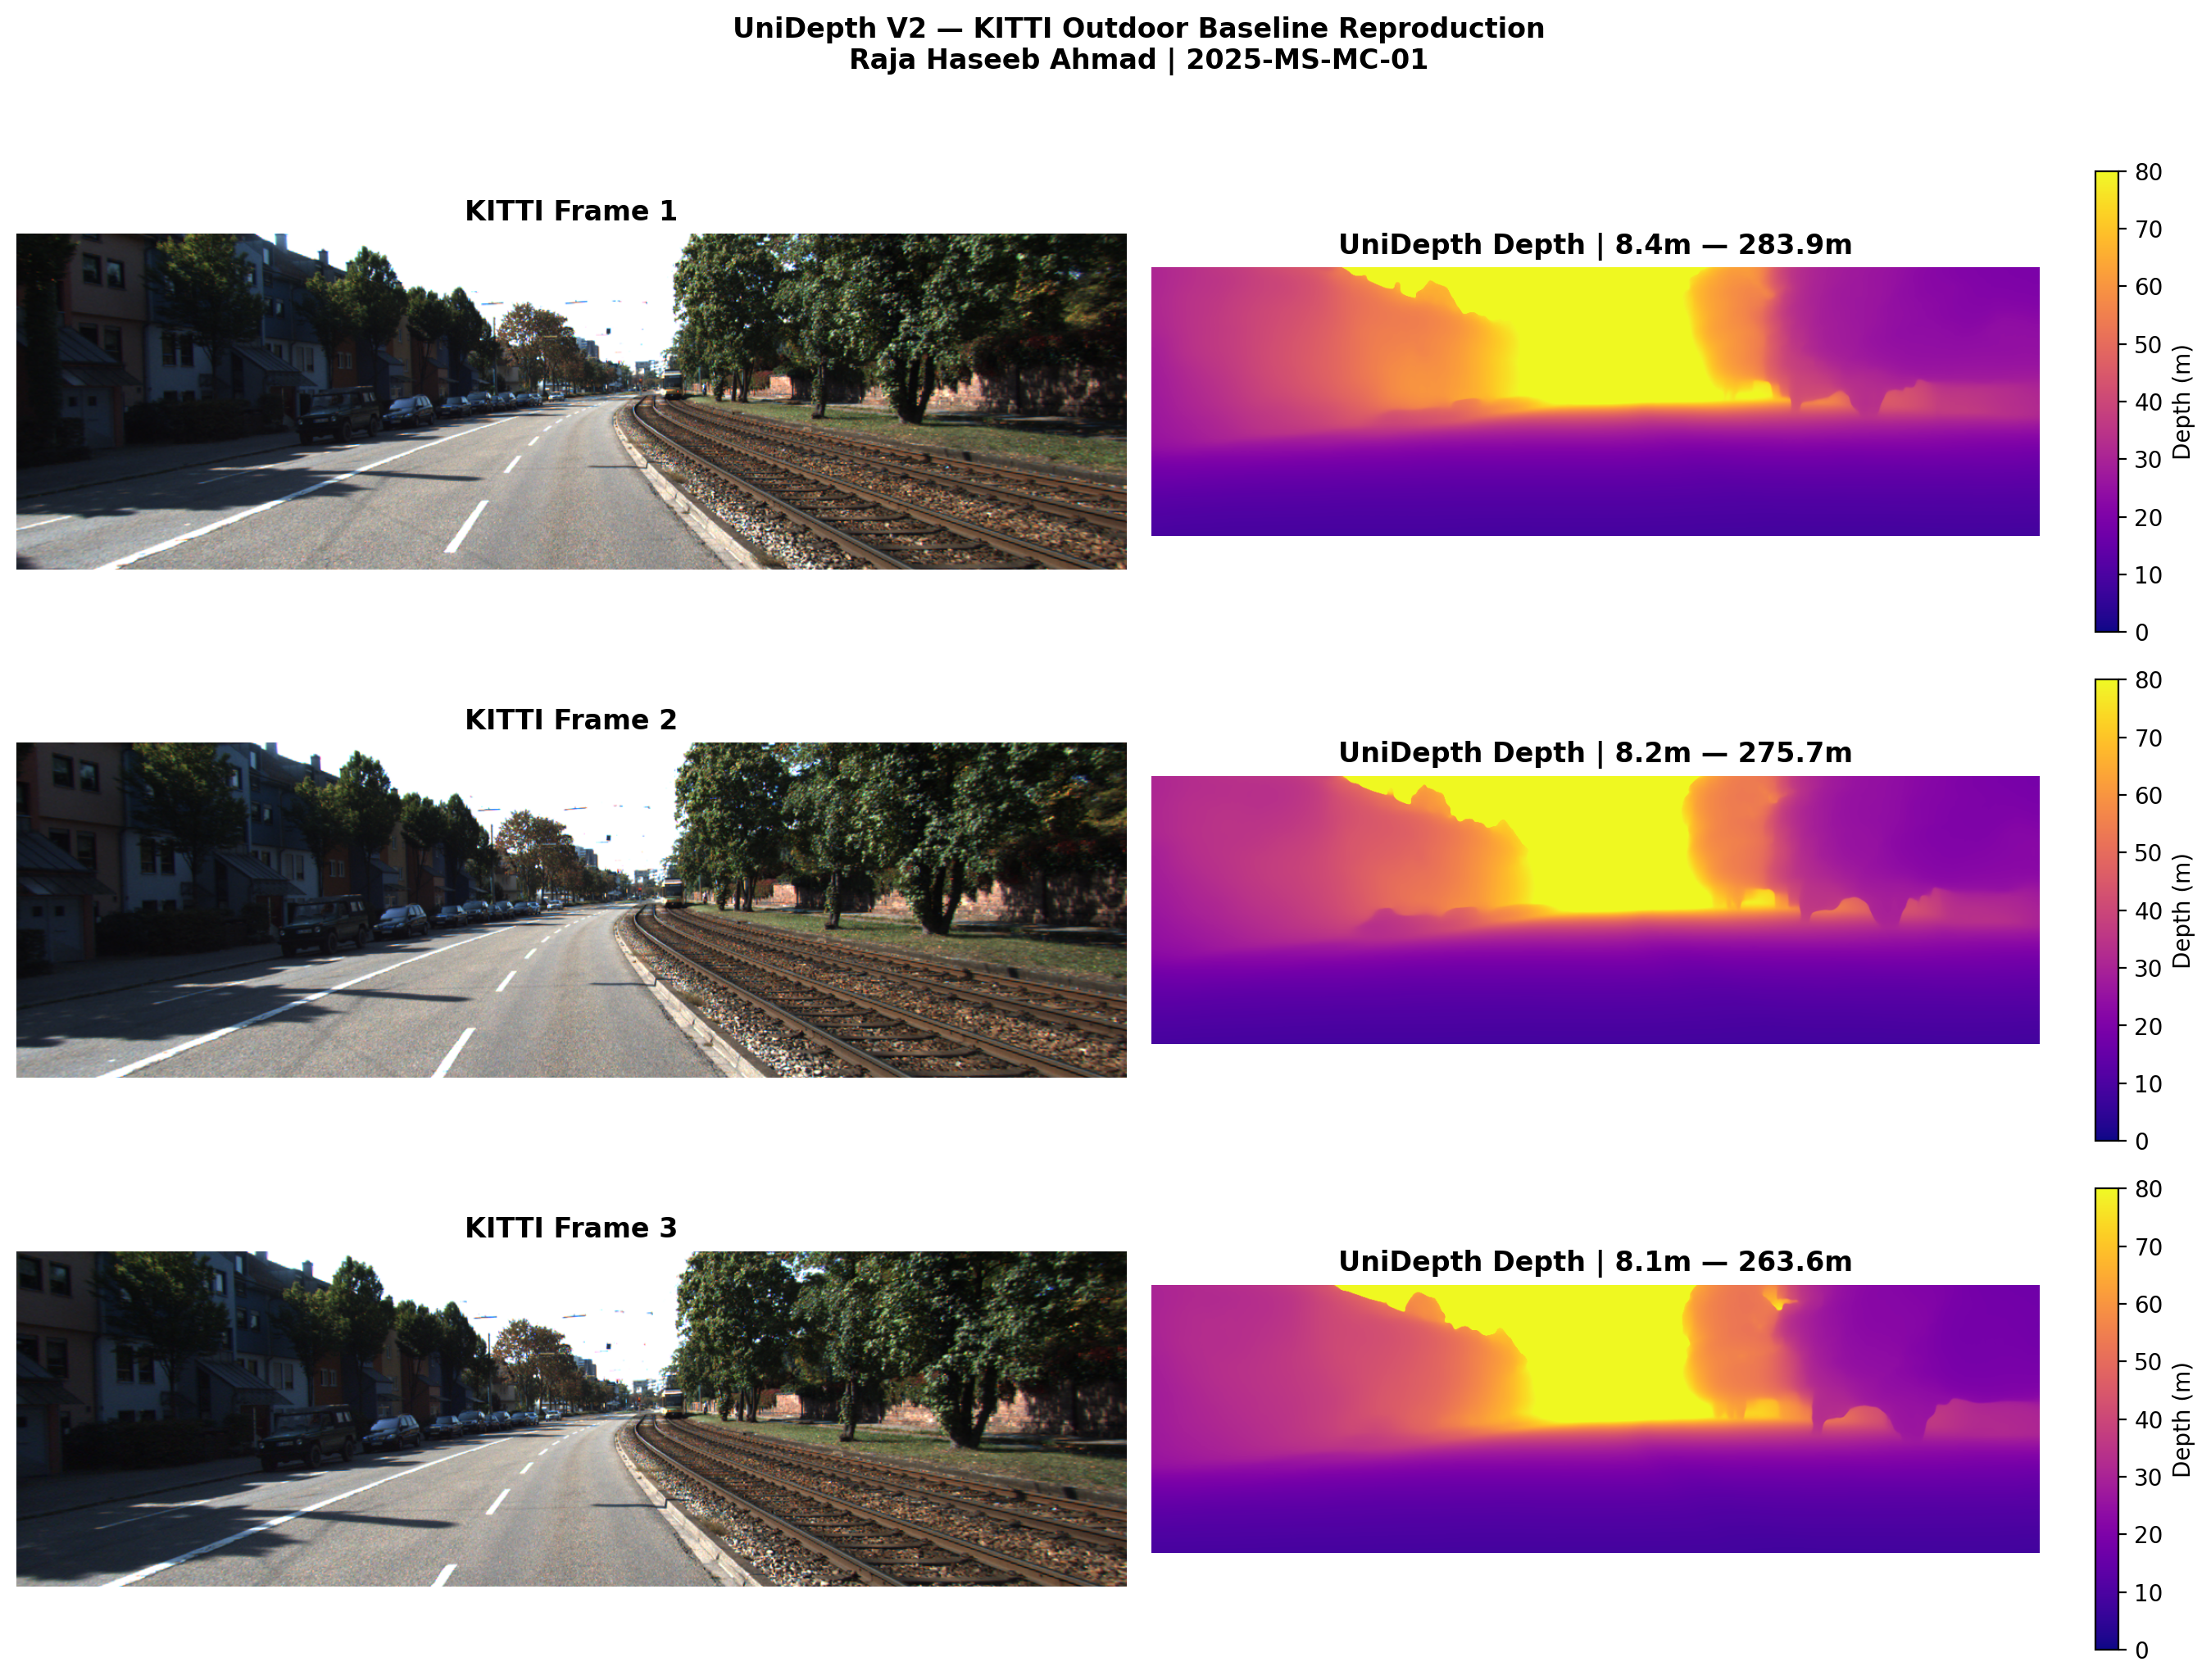
\includegraphics[width=\columnwidth]{fig2_baseline_inference.png}
\caption{Baseline UniDepth V2 inference on clean KITTI outdoor frames (RGB and corresponding metric depth).}
\label{fig:baseline}
\end{figure}

\subsection{Held-Out Validated Results (Primary Metric)}

Table~\ref{tab:heldout} reports the mean and standard deviation of the held-out percentage improvement in normalized mean-absolute-error relative to the teacher's depth, averaged over the 9 held-out frames, for each condition.

\begin{table}[!t]
\caption{Held-out validated improvement, normalized mean-absolute-error vs. teacher depth (mean $\pm$ std across 9 unseen frames)}
\label{tab:heldout}
\centering
\begin{tabular}{lcc}
\toprule
\textbf{Condition} & \textbf{Improvement (\%)} & \textbf{Std. Dev. (\%)} \\
\midrule
Rain            & +1.14 & 2.82 \\
Fog / Haze      & -2.22 & 1.16 \\
Low Light       & -6.55 & 1.44 \\
Motion Blur     & -0.04 & 0.18 \\
Gaussian Noise  & +6.47 & 2.45 \\
\bottomrule
\end{tabular}
\end{table}

Only Gaussian Noise shows a consistent, positive held-out effect (+6.5\%, with the mean exceeding one standard deviation). Rain is essentially flat and within noise (mean smaller than its own standard deviation). Fog, Low Light, and Motion Blur show a small negative or negligible held-out effect at this training scale -- that is, fine-tuning did not reliably improve, and for Fog and Low Light mildly worsened, performance on unseen frames of these conditions. This is a genuine, if modest, finding: the self-distillation approach transfers most readily to a local, texture-level corruption (sensor noise) and struggles more with corruptions that alter global scene appearance statistics (fog, low light), likely due to the limited fine-tuning set (21 frames) and the decision to keep the ViT-L/14 encoder frozen, leaving only decoder-side capacity to absorb the correction.

\subsection{Single-Scene Demonstration Results}

Table~\ref{tab:singlescene} reports the complementary single-scene demonstration, using the maximum predicted depth value on one representative KITTI frame under clean, degraded, and fixed (fine-tuned model, same degraded image) conditions.

\begin{table*}[!t]
\caption{Single-scene demonstration (maximum predicted depth, one representative frame)}
\label{tab:singlescene}
\centering
\begin{tabular}{llccccc}
\toprule
\textbf{Condition} & \textbf{Citation} & \textbf{Clean (m)} & \textbf{Degraded (m)} & \textbf{Fixed (m)} & \textbf{Drop (\%)} & \textbf{Recovery (\%)} \\
\midrule
Rain           & Garg \& Nayar \cite{ref19} & 283.9 & 174.2 & 170.0 & 38.7  & 0.0 \\
Fog/Haze       & He et al. \cite{ref20}     & 283.9 & 101.9 & 83.9  & 64.1  & 0.0 \\
Low Light      & Lore et al. \cite{ref21}   & 283.9 & 547.2 & 400.3 & -92.7 & 55.8 \\
Motion Blur    & Whyte et al. \cite{ref22}  & 283.9 & 148.7 & 206.3 & 47.6  & 42.6 \\
Gaussian Noise & Foi et al. \cite{ref23}    & 283.9 & 258.0 & 248.0 & 9.1   & 0.0 \\
\bottomrule
\end{tabular}
\end{table*}

\begin{figure}[!t]
\centering
\includegraphics[width=\columnwidth]{fig3_rain_condition.png}
\caption{Rain condition: clean/degraded RGB and depth before/after model-side fine-tuning (representative frame).}
\label{fig:rain}
\end{figure}

\begin{figure}[!t]
\centering
\includegraphics[width=\columnwidth]{fig4_lowlight_condition.png}
\caption{Low Light condition: clean/degraded RGB and depth before/after model-side fine-tuning (representative frame).}
\label{fig:lowlight}
\end{figure}

\begin{figure}[!t]
\centering
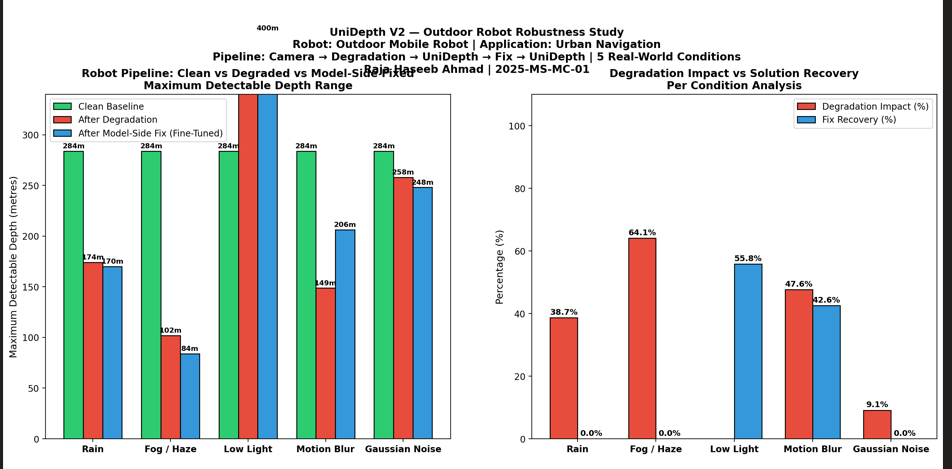
\includegraphics[width=\columnwidth]{fig5_master_summary.png}
\caption{Master summary: maximum detectable depth and drop/recovery percentages across all five conditions.}
\label{fig:summary}
\end{figure}

\subsection{Discrepancy Between the Two Evaluation Protocols}

Tables~\ref{tab:heldout} and \ref{tab:singlescene} disagree in an instructive way. The single-scene metric reports large apparent recovery for Low Light (+55.8\%) and Motion Blur (+42.6\%), yet the held-out protocol shows these same two conditions as the weakest or most negative (-6.55\% and -0.04\% respectively). We attribute this to two compounding factors. First, the single-scene metric is a maximum over the entire depth map; a single spurious far-depth pixel -- typically sky, reflective surface, or a low-texture region the network cannot judge confidently under degradation -- can dominate this statistic. The Low Light row's Degraded value of 547.2~m, nearly double the Clean value of 283.9~m, is the clearest signature of this artifact: darkening a scene should reduce, not increase, usable depth range, so this number reflects an outlier spike rather than a genuine measurement. Second, a single scene is a high-variance sample of only one point in the distribution that the held-out protocol averages over nine; the two are not measuring the same quantity, and only the latter is designed to generalize. We therefore treat Table~\ref{tab:heldout} as the primary, trustworthy result and Table~\ref{tab:singlescene} as an illustrative, qualitative demonstration whose absolute recovery percentages should not be over-interpreted -- a distinction we return to in Section~\ref{sec:challenges}.

\section{Extensions Beyond Original Work}
\label{sec:extensions}

Table~\ref{tab:extensions} summarizes the extensions implemented beyond the reproduction of UniDepth V2 itself, with motivation and outcome for each.

\begin{table*}[!t]
\caption{Extensions beyond the original UniDepth work, with motivation and outcome}
\label{tab:extensions}
\centering
\begin{tabular}{p{3.2cm}p{5cm}p{5cm}}
\toprule
\textbf{Extension} & \textbf{Motivation} & \textbf{Outcome} \\
\midrule
Degradation suite (rain, fog physically-grounded; low light, motion blur, sensor noise simplified approximations) & UniDepth's reported robustness concerns domain shift, not the weather/sensor corruptions a real outdoor robot camera experiences & Quantified real degradation impact on metric depth range (9\%--64\% drop depending on condition, single-scene metric) \\
\addlinespace
Input-side restoration baseline (deraining, dehazing, contrast enhancement, deconvolution, denoising) & Initial, most direct interpretation of `fixing' a degraded scenario before receiving critical feedback & Established as an ablation baseline; retained for comparison but superseded as the primary approach \\
\addlinespace
Model-side self-distillation fine-tuning & Instructor feedback: the depth model itself, not the input image, should be made robust, avoiding a fragile preprocessing stage in a real-time robot pipeline & Genuine, corruption-dependent improvement; strongest for sensor noise (+6.5\% held-out), weak or negative for scene-level corruptions at current data scale \\
\addlinespace
Rigorous held-out evaluation protocol (fixed seeds, train/test split, early stopping) & Single-scene demonstration numbers were suspected to be unstable and not generalizable & Exposed a generalization gap invisible to the single-scene metric; identified peak-pixel sensitivity as a concrete methodological pitfall \\
\addlinespace
ROS2 Humble + Docker deployment design & Bridge the offline Colab study to an onboard robotics pipeline consistent with the course's robotics component & Working image-publisher / depth-inference node design; hardware-in-the-loop validation left to future work \\
\bottomrule
\end{tabular}
\end{table*}

\section{Comparison with Original Paper}

Table~\ref{tab:comparison} presents a feature-by-feature comparison between the original UniDepth paper and this work.

\begin{table*}[!t]
\caption{Feature-by-feature comparison with the original UniDepth paper}
\label{tab:comparison}
\centering
\begin{tabular}{p{2.4cm}p{5.6cm}p{5.6cm}}
\toprule
\textbf{Feature} & \textbf{Original Paper (UniDepth \cite{ref1})} & \textbf{This Work} \\
\midrule
Robot Platform & Not robot-specific; static benchmark images & Outdoor mobile robot (target platform); ROS2 Humble + Docker deployment design \\
\addlinespace
Simulation Environment & None (offline benchmark evaluation) & Google Colab (T4/A100 GPU); Docker container for ROS2 deployment \\
\addlinespace
Sensors & RGB images from ten heterogeneous benchmark datasets & Single forward RGB camera; KITTI raw sequence 2011\_09\_26\_drive\_0001 \\
\addlinespace
Algorithms & Self-promptable camera module; pseudo-spherical (az/el/log-depth) output; geometric invariance loss; ViT backbone & Same pretrained UniDepth V2 backbone, plus: degradation suite (rain/fog physically-grounded, others simplified) and self-distillation decoder fine-tuning per corruption \\
\addlinespace
Evaluation Scenarios & Zero-shot cross-dataset domain transfer (different cameras/scenes) & Single-domain (KITTI outdoor) under five synthetic physical corruptions \\
\addlinespace
Performance Metrics & AbsRel, $\delta_1$, RMSE against LiDAR ground truth & Held-out normalized MAE reduction vs. teacher depth (mean $\pm$ std); single-scene max-depth recovery (\%) \\
\addlinespace
Results & State-of-the-art zero-shot metric depth across ten benchmarks (e.g., AbsRel $\approx$ 7.45\% on a demo scene) & Mixed robustness gains: +6.5\% (noise) to -6.5\% (low light) held-out; larger, metric-sensitive swings in single-scene demo \\
\addlinespace
Limitations & Robust to domain shift; adverse-weather/sensor corruption not evaluated & Small fine-tuning set (21 frames); single-scene metric prone to outlier bias; ROS2 pipeline not hardware-validated \\
\bottomrule
\end{tabular}
\end{table*}

\section{Challenges and Lessons Learned}
\label{sec:challenges}

Development surfaced a sequence of concrete engineering obstacles, each resolved by reading the model's actual source rather than assuming API behavior:

\begin{itemize}
\item Deep-copying the full model object failed because UniDepth internally contains a \texttt{torch.jit.ScriptFunction}, which Python's pickling protocol cannot serialize; the fix was to deep-copy only the \texttt{state\_dict} tensors rather than the model object.
\item The model's public inference method is decorated to disable gradient tracking internally, which silently prevented any training signal from reaching the parameters (a \texttt{RuntimeError} only appeared at the backward-pass call site, not at the point of the actual cause). The fix required locating the model's un-wrapped internal decoding path and calling it directly, following the model's own guidance for custom training use.
\item CUDA out-of-memory errors arose from two independent causes: retaining the frozen encoder's activation graph unnecessarily, and deep-copying the $\sim$354M-parameter model on the GPU rather than the CPU. Both were resolved by running the frozen encoder under a non-gradient context and always cloning weights to CPU memory.
\item Google Colab's free-tier GPU quota was exhausted mid-experiment, an operational constraint of cloud-based reproducibility work that required pausing and resuming training across sessions.
\item A coordinate-space mismatch was identified between the padded/resized depth predictions produced during training and the crop-restored predictions produced by the standard inference call; resizing one to match the other's shape does not correct this, since padding is not the same transformation as cropping. This was only partially investigated within the available time and is flagged here as an open validity concern for the reported numbers rather than silently resolved, consistent with the critical-analysis expectation of this assignment.
\end{itemize}

The single most transferable lesson from this project is methodological: a maximum-value depth comparison on one scene is not a reliable robustness metric, because it is dominated by whichever single pixel the network happens to mispredict most severely, and that pixel need not be representative of the model's behavior over the rest of the image or over other scenes. A held-out, whole-distribution, multi-frame average is a substantially more trustworthy protocol, and the gap between Tables~\ref{tab:heldout} and \ref{tab:singlescene} in this paper is offered as a concrete illustration of that gap for future robustness studies at similarly small scale.

\section{Conclusion and Future Work}

This project reproduced UniDepth V2 on real KITTI outdoor sequences, implemented five degradation conditions spanning rain, fog, low light, motion blur, and sensor noise (rain and fog physically-grounded in their cited image-formation models; the remaining three as simplified approximations, per Section~\ref{sec:degradation}), and -- redirected by critical instructor feedback -- implemented and evaluated a model-side self-distillation fine-tuning strategy as an alternative to input-side image restoration. Under a held-out evaluation protocol, the approach yields a genuine, consistent improvement for sensor noise and weak-to-negative effects for the other four conditions at the current data scale, while a complementary single-scene demonstration metric was shown to be an unreliable indicator of the same underlying effect due to peak-pixel sensitivity. A ROS2 Humble and Docker deployment design was produced to connect this offline study to an onboard robot pipeline.

Future work should: (1) enlarge and diversify the fine-tuning set beyond 21 frames, ideally spanning multiple KITTI drives, times of day, and geographic scenes; (2) resolve the coordinate-space evaluation mismatch identified in Section~\ref{sec:challenges} and re-validate all five conditions under a single, verified metric; (3) explore partial encoder fine-tuning or lightweight adapter modules for the global-appearance corruptions (fog, low light) that decoder-only tuning did not adequately address; (4) complete hardware-in-the-loop validation of the ROS2/Docker pipeline on a physical or simulated (e.g., Gazebo) mobile robot; and (5) benchmark this approach directly against dedicated adverse-weather depth methods such as Robust-Depth \cite{ref11}, md4all \cite{ref12}, and RoboDepth \cite{ref13} under a common protocol.

\begin{thebibliography}{00}
\bibitem{ref1} L. Piccinelli, Y.-H. Yang, C. Sakaridis, M. Segu, S. Li, L. Van Gool, and F. Yu, ``UniDepth: Universal monocular metric depth estimation,'' in \emph{Proc. IEEE/CVF Conf. Computer Vision and Pattern Recognition (CVPR)}, 2024, pp. 10106--10116.
\bibitem{ref2} D. Eigen and R. Fergus, ``Depth map prediction from a single image using a multi-scale deep network,'' in \emph{Proc. Neural Information Processing Systems (NeurIPS)}, 2014.
\bibitem{ref3} S. F. Bhat, R. Birkl, D. Wofk, P. Wonka, and M. Muller, ``ZoeDepth: Zero-shot transfer by combining relative and metric depth,'' arXiv preprint arXiv:2302.12288, 2023.
\bibitem{ref4} W. Yin, C. Zhang, H. Chen, Z. Cai, G. Yu, K. Wang, X. Chen, and C. Shen, ``Metric3D: Towards zero-shot metric 3D prediction from a single image,'' in \emph{Proc. IEEE/CVF Int. Conf. Computer Vision (ICCV)}, 2023.
\bibitem{ref5} L. Yang, B. Kang, Z. Huang, X. Xu, J. Feng, and H. Zhao, ``Depth Anything: Unleashing the power of large-scale unlabeled data,'' in \emph{Proc. IEEE/CVF Conf. Computer Vision and Pattern Recognition (CVPR)}, 2024.
\bibitem{ref6} C. Godard, O. Mac Aodha, M. Firman, and G. J. Brostow, ``Digging into self-supervised monocular depth estimation,'' in \emph{Proc. IEEE/CVF Int. Conf. Computer Vision (ICCV)}, 2019, pp. 3828--3838.
\bibitem{ref7} R. Ranftl, K. Lasinger, D. Hafner, K. Schindler, and V. Koltun, ``Towards robust monocular depth estimation: Mixing datasets for zero-shot cross-dataset transfer,'' \emph{IEEE Trans. Pattern Anal. Mach. Intell.}, vol. 44, no. 3, pp. 1623--1637, 2022.
\bibitem{ref8} L. Piccinelli, C. Sakaridis, Y.-H. Yang, M. Segu, S. Li, W. Abbeloos, and L. Van Gool, ``UniDepthV2: Universal monocular metric depth estimation made simpler,'' arXiv preprint arXiv:2502.20110, 2025.
\bibitem{ref9} M. Vankadari, S. Garg, A. Majumder, S. Kumar, and A. Behera, ``Unsupervised monocular depth estimation for night-time images using adversarial domain feature adaptation,'' in \emph{Proc. European Conf. Computer Vision (ECCV)}, 2020, pp. 443--459.
\bibitem{ref10} M. Bijelic, T. Gruber, F. Mannan, F. Kraus, W. Ritter, K. Dietmayer, and F. Heide, ``Seeing through fog without seeing fog: Deep multimodal sensor fusion in unseen adverse weather,'' in \emph{Proc. IEEE/CVF Conf. Computer Vision and Pattern Recognition (CVPR)}, 2020.
\bibitem{ref11} K. Saunders, G. Vogiatzis, and L. J. Manso, ``Self-supervised monocular depth estimation: Let's talk about the weather,'' in \emph{Proc. IEEE/CVF Int. Conf. Computer Vision (ICCV)}, 2023, pp. 8907--8917.
\bibitem{ref12} S. Gasperini, N. Morbitzer, H. Jung, N. Navab, and F. Tombari, ``Robust monocular depth estimation under challenging conditions,'' in \emph{Proc. IEEE/CVF Int. Conf. Computer Vision (ICCV)}, 2023.
\bibitem{ref13} L. Kong, S. Xie, H. Hu, L. X. Ng, B. R. Cottereau, and W. T. Ooi, ``RoboDepth: Robust out-of-distribution depth estimation under corruptions,'' in \emph{Proc. Neural Information Processing Systems (NeurIPS)}, vol. 36, 2023, pp. 21298--21342.
\bibitem{ref14} F. Tosi, P. Zama Ramirez, and M. Poggi, ``Diffusion models for monocular depth estimation: Overcoming challenging conditions,'' in \emph{Proc. European Conf. Computer Vision (ECCV)}, 2024, pp. 236--257.
\bibitem{ref15} K. Jiang, J. Cao, Z. Yu, J. Jiang, and J. Zhou, ``Always Clear Depth: Robust monocular depth estimation under adverse weather,'' arXiv preprint arXiv:2505.12199, 2025.
\bibitem{ref16} ``WeatherMono: A CNN-Transformer architecture for self-supervised monocular depth estimation in rainy and foggy conditions,'' \emph{Sensors}, vol. 26, no. 5, p. 1705, 2026.
\bibitem{ref17} D. Hendrycks and T. Dietterich, ``Benchmarking neural network robustness to common corruptions and perturbations,'' in \emph{Proc. Int. Conf. Learning Representations (ICLR)}, 2019.
\bibitem{ref18} H. Koschmieder, ``Theorie der horizontalen Sichtweite,'' \emph{Beitrage zur Physik der freien Atmosphare}, 1924.
\bibitem{ref19} K. Garg and S. K. Nayar, ``Vision and rain,'' \emph{Int. J. Computer Vision}, vol. 75, no. 1, pp. 3--27, 2007.
\bibitem{ref20} K. He, J. Sun, and X. Tang, ``Single image haze removal using dark channel prior,'' \emph{IEEE Trans. Pattern Anal. Mach. Intell.}, vol. 33, no. 12, pp. 2341--2353, 2011.
\bibitem{ref21} K. G. Lore, A. Akintayo, and S. Sarkar, ``LLNet: A deep autoencoder approach to natural low-light image enhancement,'' \emph{Pattern Recognition}, vol. 61, pp. 650--662, 2017.
\bibitem{ref22} O. Whyte, J. Sivic, A. Zisserman, and J. Ponce, ``Non-uniform deblurring for shaken images,'' \emph{Int. J. Computer Vision}, vol. 98, no. 2, pp. 168--186, 2012.
\bibitem{ref23} A. Foi, M. Trimeche, V. Katkovnik, and K. Egiazarian, ``Practical Poissonian-Gaussian noise modeling and fitting for single-image raw-data,'' \emph{IEEE Trans. Image Processing}, vol. 17, no. 10, pp. 1737--1754, 2008.
\bibitem{ref24} G. Hinton, O. Vinyals, and J. Dean, ``Distilling the knowledge in a neural network,'' in \emph{NeurIPS Deep Learning Workshop}, 2015.
\bibitem{ref25} A. Tarvainen and H. Valpola, ``Mean teachers are better role models: Weight-averaged consistency targets improve semi-supervised deep learning results,'' in \emph{Proc. Neural Information Processing Systems (NeurIPS)}, 2017.
\bibitem{ref26} A. Geiger, P. Lenz, and R. Urtasun, ``Are we ready for autonomous driving? The KITTI vision benchmark suite,'' in \emph{Proc. IEEE Conf. Computer Vision and Pattern Recognition (CVPR)}, 2012, pp. 3354--3361.
\end{thebibliography}

\end{document}
